\section{Theorie}
\label{sec:Theorie}
\subsection{Austritsarbeit und Energieverteilung von Elektronen}
Metalle sind kristalline Festkörper. Sie bilden ein Gitter von 
Ionisierten Athomen, welches von nahezu Kräftefrei bewegten Elektronen 
eingehüllt wird. Kräftefrei ist es daher, da im inneren des Metalles das "Gitterpotential"
nahezu konstant ist, sodass sich die Elektronen dort frei bewegen Können. Um Elektronen jedoch 
aus dem Metall zu emmitieren muss eine Austritsarbeit überwunden werden, da das Potential auserhalb 
des Metalls verschieden ist.
\begin{figure}[H]
    \centering
        \centering
        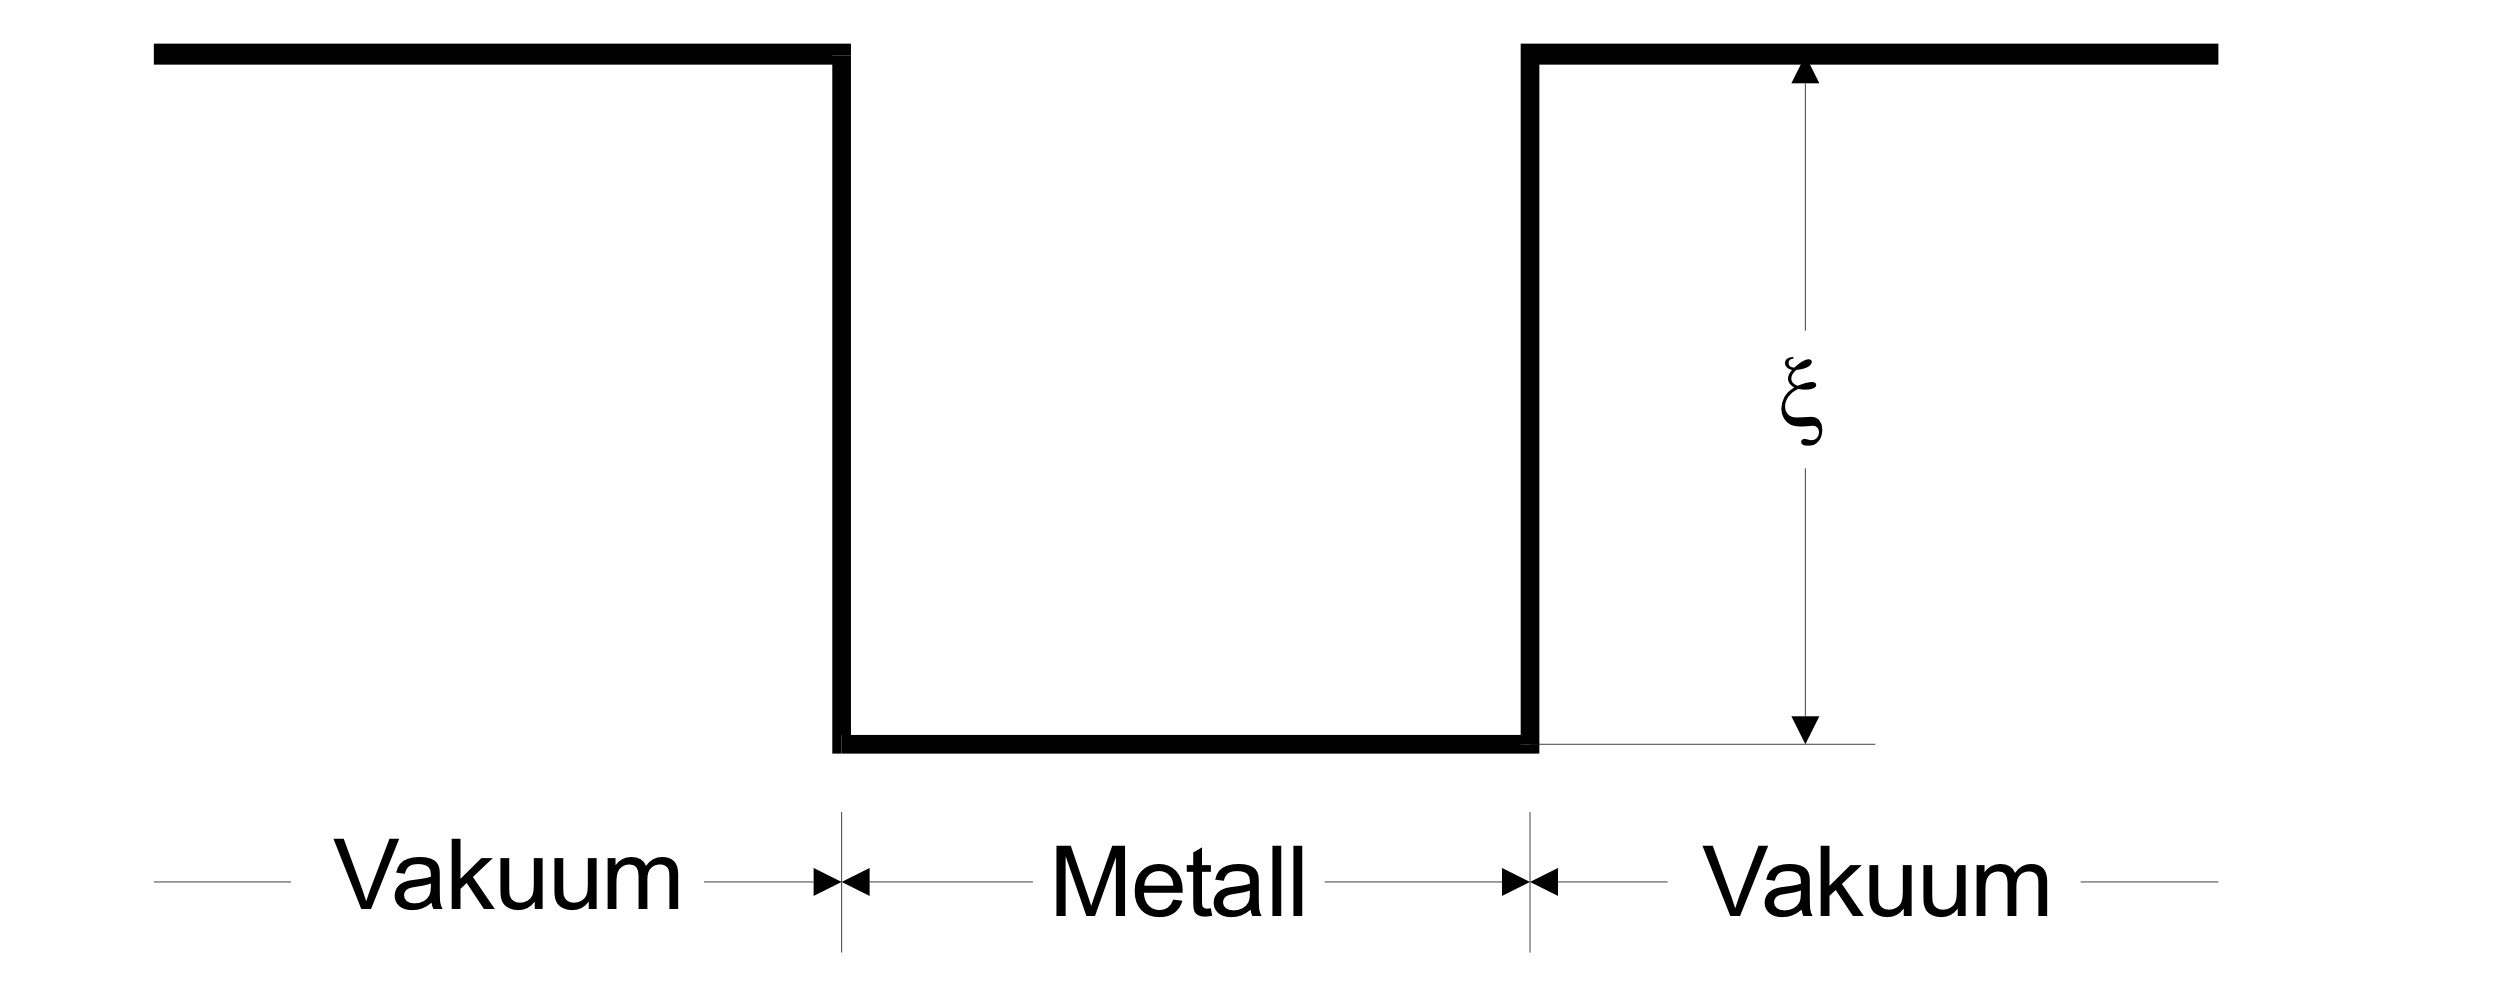
\includegraphics[width=\textwidth]{Bilder/potentialtopf.jpg}
        \caption{Potentialtopf-Modell eines Metalls}
    \hfill
    \label{fig:phasendiagramm}
\end{figure}
Anhand des Potentialtopfmodells lässt sich verdeutlichen, dass die Elektronen eine Austritsarbeit von 
$\exp _0 \xi$ verrichten muss.

Elektronen unterliegen dem Pauli Prinzip, das bedeutst nur Elektronen mit entgegengesetzten Spinstellungen können einen möglichen Zustand besetzen. 
Somit wird die Energieverteilung der Elektronen in einem Metall durch die Fermi-Dirac verteilung beschrieben.

\begin{equation}
    \label{eqn:1}
    f\left(E\right) = \frac{1}{\exp{\frac{\zeta-E}{k_b T} + 1}}
\end{equation}
\noindent in \autoref{eqn:1} ist die Fermi-Dirak Verteilungsfunktion mit der Fermi-Energie $\zeta$ gegeben. Diese kann 
für eine hohe Energie $\zeta$, welche die Austritsarbeit überwinden kann, genähert werden. die Näherung ist in \autoref{eqn:2} 
gegeben. Des weiteren ist der Verlauf der Verteilungsfunktion in \autoref{fermi} dargestellt.
\begin{equation}
    \label{eqn:2}
    f\left(E\right) \approx \exp{\frac{\zeta-E}{k_b T}}
\end{equation}
\begin{figure}[H]
    \centering
        \centering
        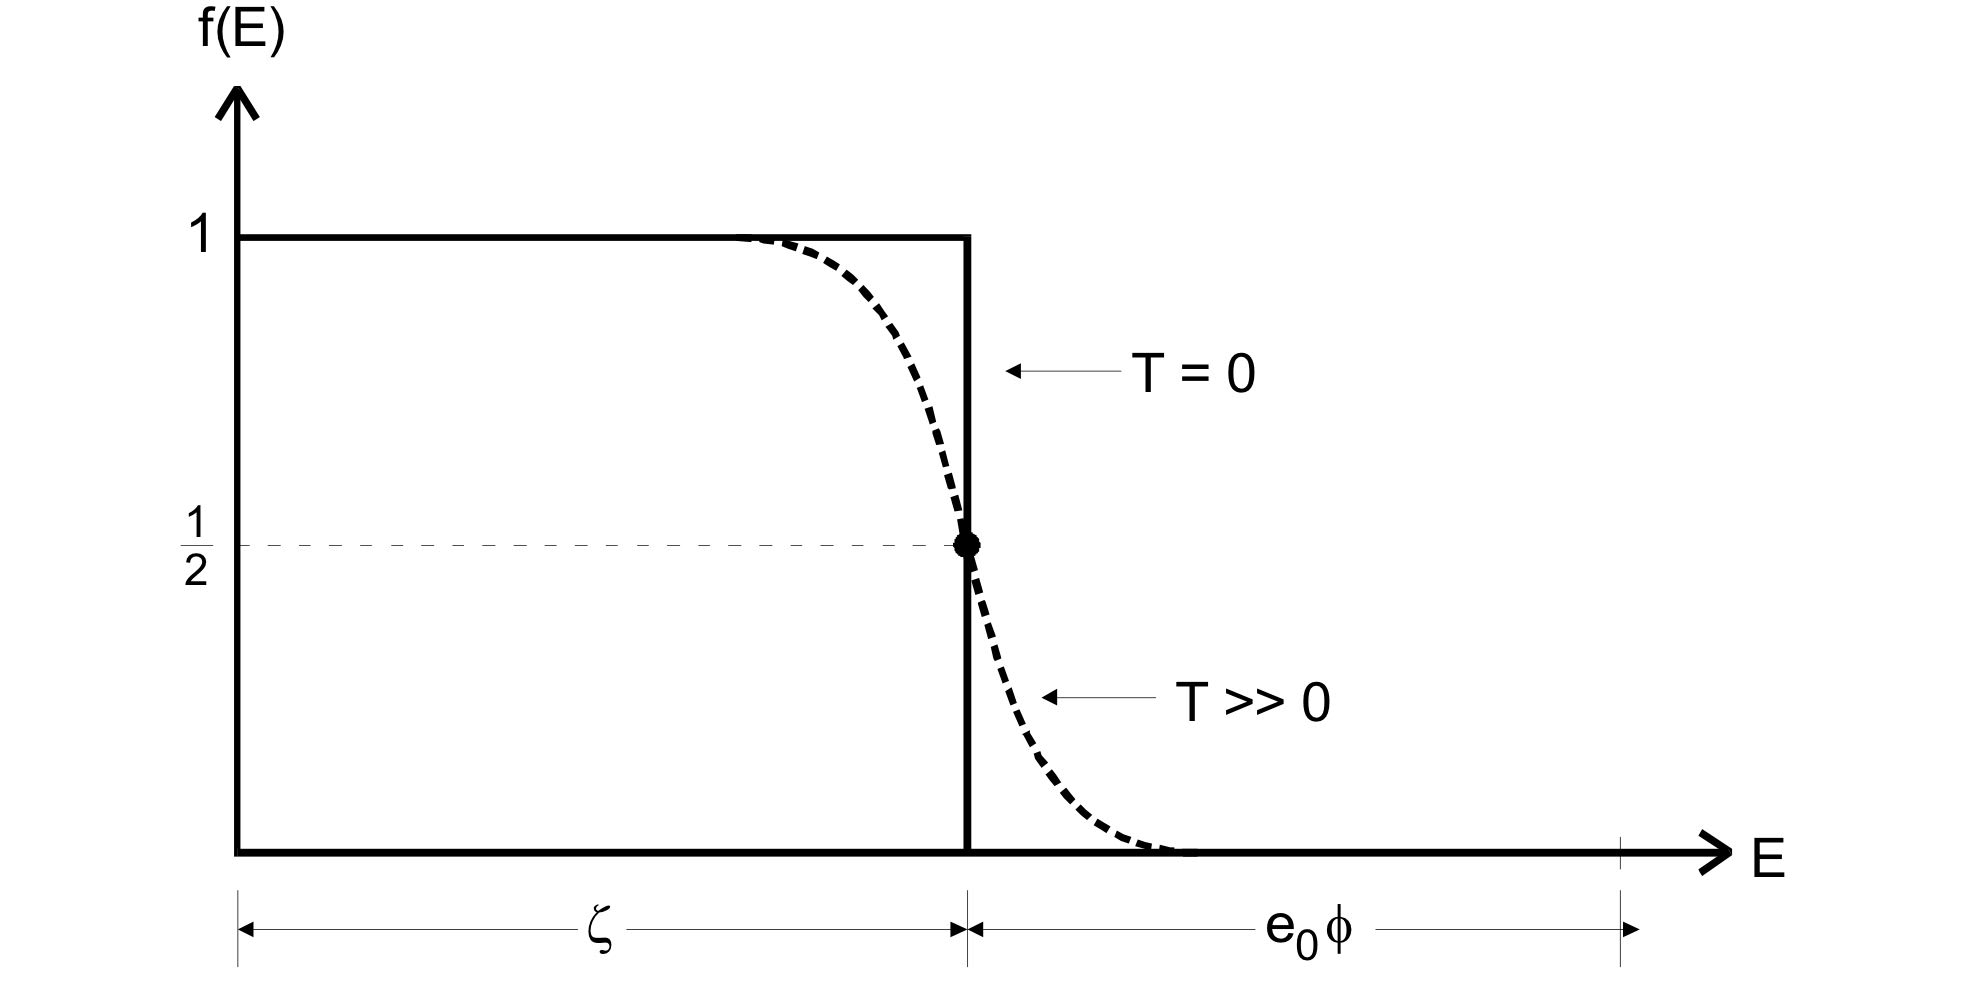
\includegraphics[width=\textwidth]{Bilder/Fermi-Dirac.jpg}
        \caption{Fermi-Dirak Verteilung}
    \hfill
    \label{fig:fermi}
\end{figure}

\subsection{Sättigungsstromdichte der Thermischen elektronenemission}
Mithilfe von \autoref{eqn:2} kann man auf einen Ausdruck für die zahl der Elektronen pro zeit schließen, welche 
aus dem metall austreten. Diese zahl ist Abhängig von der Temperatur des Metalls und wird duch die Richardson Gleichung 
in \autoref{eqn:3} beschrieben.
\begin{equation}
    \label{eqn:2}
    J_s \left(T\right) = 4\pi \frac{e_0m_0k^2}{h^3}T^2\exp{\frac{-e_0\Phi}{k_b T}}
\end{equation}


\subsection{DIe Hochvakuum Diode und Langmuir-Schottkysche Raumladungsgleichung}
Um die austretenden Elektronen zu messen, muss Das Metall in ein Vakuum gebracht werden, damit die elektronen nit mit Gasmolekülen wechselwirken würden. 
Im Vakuum können sie durch ein Angelegtes Spannungsfeld zu einer Anode abgesaugt werden. Somit kommt eine Hochvakuumdiode in \autoref{fig:3}
zum Einsatz.
\begin{figure}[H]
    \centering
        \centering
        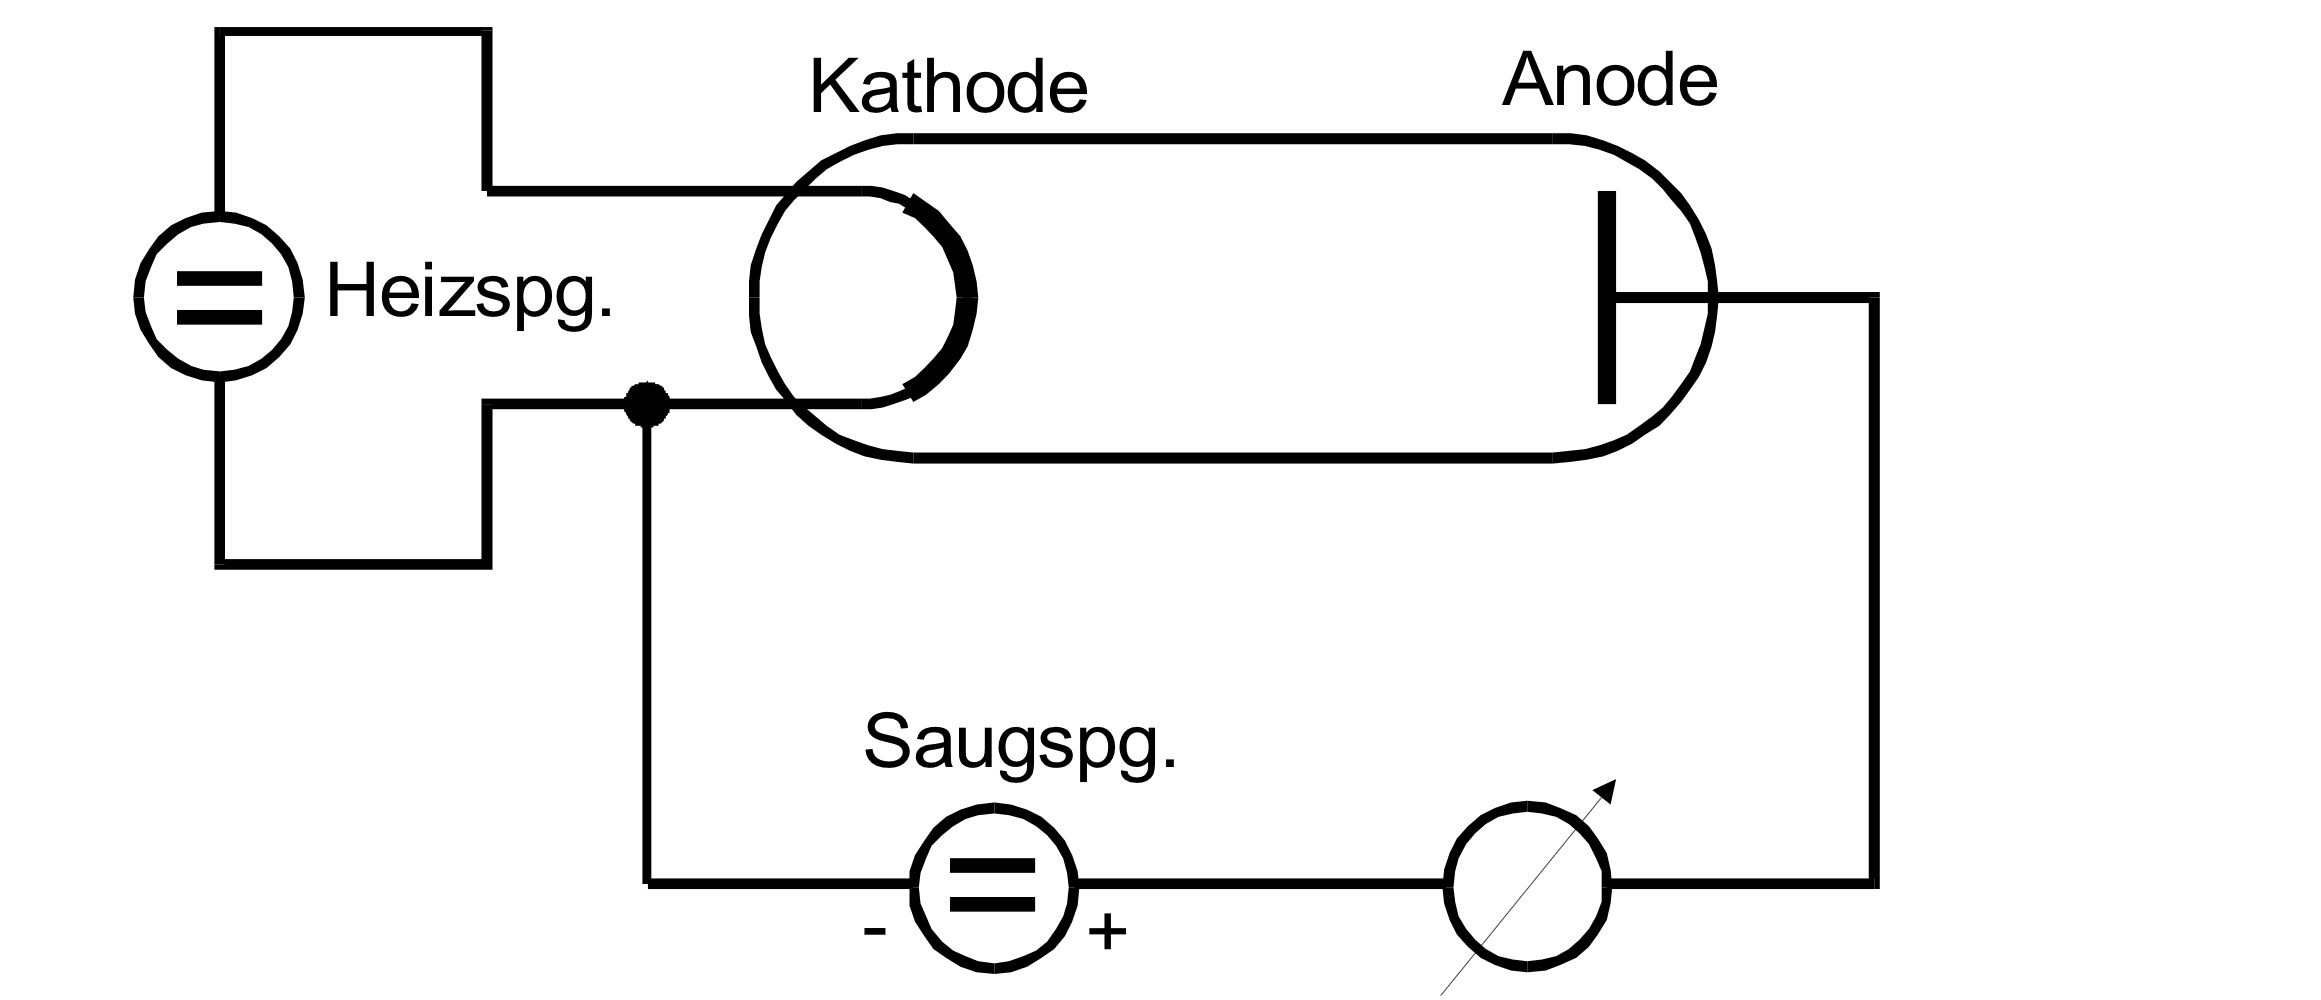
\includegraphics[width=\textwidth]{Bilder/schaltung.jpg}
        \caption{Schaltung einer Hochvakuum-Diode}
    \hfill
    \label{fig:3}
\end{figure}
Die "Absaugung" der Elektronen zur Positiv geladenen Anode hin führt jedoch dazu, dass die Elektronen, je näher sie an 
die Anode rankommen, höher beschleunigt werden. Dadurch haben eine höhere Geschwindigkeit je näher sie der Anode kommen. 
Durch die kontinuitätsbedingung der Stromdichte $j$ 
\begin{equation}
j = -\rho v
\end{equation}
,mit der Stromdichte $j$ und der Raumladungsdichte $\rho$, führt nun die unterschiedliche Geschwindigkeitsverteilung in der Vakuum diode 
auch zu einer Ladungsverteilung, welche von der Kathode hin zur anode abnimmt. Durch die unterschiedliche Ladungsdichte wird die Kathode und nicht mehr alle Feldlinien
 ausgehend von der Anode erreichen die Kathode. Damit ist der gemessene Diodenstrom kleiner als der erwartete Sättigungsstrom.
